\documentclass[12pt]{article}                         % Make it an article
\usepackage{indentfirst}                       % All paragraphs indented
\usepackage{setspace}                           % For 1.5 spacing
\usepackage[hidelinks]{hyperref}      % Make table of contents clickable
\usepackage[margin=1in]{geometry} % 1 inch margin
\usepackage[english]{babel}                     % For "fancy" quotes
\usepackage[autostyle, english=american]{csquotes} % Same
\usepackage{apacite}                            % Use APA citations
\usepackage{etoolbox}                           % Misc
\usepackage{titlesec}
\usepackage{listofauthorships}
\MakeOuterQuote{"}                              % For fancy quotes
\usepackage{times}                              %For Tilde
\usepackage{textcomp}                           %For Tilde
\usepackage{graphicx}                           %Images
\graphicspath{{./images/}}
\titlespacing*{\section}{0pt}{0pt}{0pt}
\titlespacing*{\subsection}{0pt}{0pt}{0pt}
\titlespacing*{\subsubsection}{0pt}{5pt}{-3pt}

\title{Eilat: Transportation 2040}
\author{Evan Goldstein, Valeria Kopper, Christopher Myers, Zachary Zlotnick}
\date{\today}

\begin{document}
\pagenumbering{gobble}
\maketitle

\vspace{12cm}
\begin{minipage}{0.5\textwidth}
    \begin{flushleft} \large
        
\includegraphics[width=2.5cm]{eilat_logo.png} \\
        \textbf{Sponsored by:} \\
        A. Adamon, \\
        E. Toppel \\
        \textit{Eilat Municipality}
    \end{flushleft}
\end{minipage}
~
\begin{minipage}{0.4\textwidth}
    \begin{flushright} \large
        
\includegraphics[width=5.5cm]{WPI_logo.png} \\
        \vspace{0.7cm}
        \textbf{Submitted to:}\\
        Professor Bar-On
        \vspace{1.5cm}
    \end{flushright}
\end{minipage}

\newpage

\renewcommand\abstractname{Summary} % "Abstract" -> "Summary", the header lies

\pagenumbering{roman}
\tableofcontents
\newpage
\listofauthorships
\newpage
\pagenumbering{arabic}
\doublespacing

% Actual content begins here!
\section{Introduction}[All]

Eilat is a city in the southern tip of Israel with a growing population of ~50,000 and an area of 85 km$^2$. The city is a popular tourist destination, with over 3 million tourists per year from around the world. Given past trends, tourism is expected to continue increasing in the future.

The city currently suffers from heavy congestion at peak hours, and the new Ramon airport on route 90 is expected to worsen the situation, increasing travel times. This compounded congestion will put a strain on Eilat's transport network, calling for an increased effort to shorten commute times, expand Eilat's transportation services, and streamline the travel experience.

Understanding current constraints for transportation in Eilat will allow for planning what future transportation will look like in the city, and the implementation of certain smart city initiatives. For example, these initiatives would include the implementation of sensors that would allow for smart traffic management. Overall, smart city technologies aim to help modernize city functions as well as improve quality of life for residents, tourists, and businesses.

Currently, Egged operates intra-city buses in Eilat. A bus ride from the west side of the city to the airport takes about 26 minutes with no traffic, and from Yotam Square to the hotels zone is 35 minutes. These lengthy travel times are due to a high number of stops across a wide area. Other transportation options such as trams have not been previously considered, and could replace buses or work alongside them to decrease travel times. Less invasive options such as public bikes and scooters have also not been thoroughly investigated.

The goal of this project is to aid the city of Eilat in investigating possible transportation services that minimize environmental impact, congestion, and travel times for residents, tourists, and businesses while improving ease of travel. To accomplish this, we will first develop a detailed understanding of Eilat's current transport network, its requirements, advantages, and disadvantages. We will then create predictions for future congestion in the city based on projected growth and currently planned transportation changes. We will produce a roadmap to guide Eilat's transportation development through 2040 and present data on current and future transport. An optimized transportation network will improve the lives of residents and tourists, and the economy in Eilat.
 
\newpage
\section{Background}

\subsection{Existing Transportation}[Chris M., Zach Z.]

\begin{figure}[h]
    \centering
    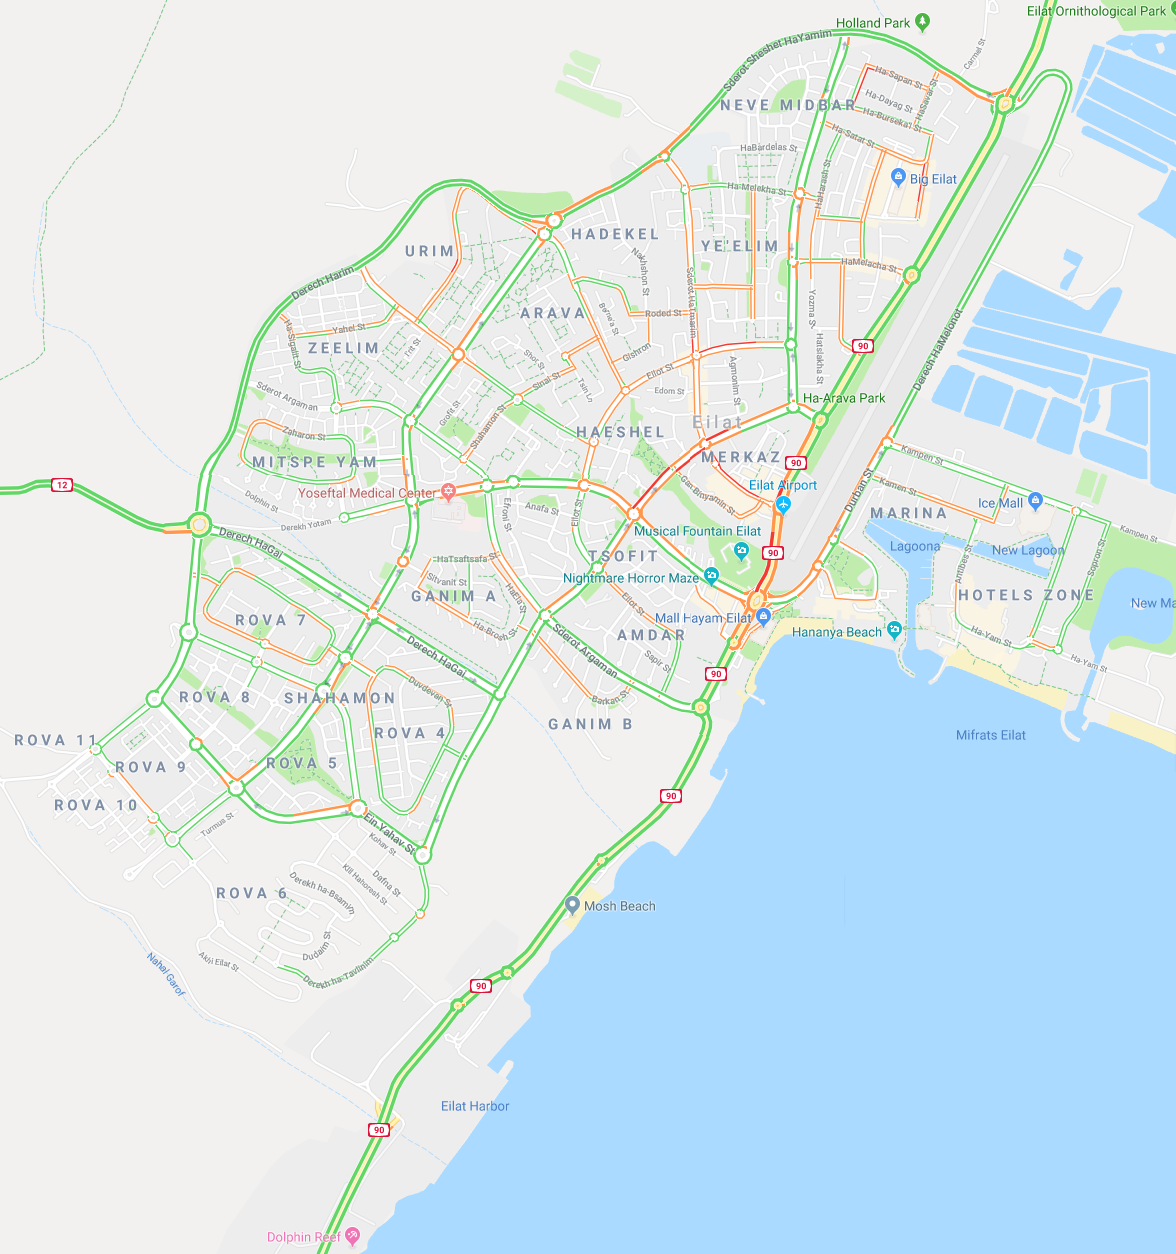
\includegraphics[scale=1]{eilat_traffic.png}
    \caption{Traffic map of Eilat at 5 PM weekdays (off-season)}
    \label{img:eilatTraffic}
\end{figure}

Israel's route 90 is the main road leading into Eilat, seen in the top right of figure \ref{img:eilatTraffic}, and is subject to heavy congestion during the tourism season, especially during peak hours. Red and orange roads indicate heavy and moderate congestion, respectively. During rush hours, congestion is moderate in most major city arteries even off-season. A notable hotspot is the Eilat airport (on the center right) which travelers frequently enter and exit. However, this airport is set to shut down as Ramon Airport opens later this year along route 90, and Ovda Airport (which feeds into route 12 on the far left) will stop handling civilian flights. This leaves Ramon airport as the only airport servicing Eilat, creating a focal point for congestion wherever route 90 meets with city roads. Given the already evident congestion, major traffic jams and increased travel times can be expected.

Alternatives to conventional public methods of transportation already exist to bridge the gaps in commuting. "Bird" has successfully implemented an electric scooter system in over 100 cities worldwide, solving public transport's "last mile" problem. Riders pick up a scooter from any "nest" in the city and pay an initial fee plus a fixed fee for each minute used \cite{MichaelRaz-Chaimovich2018BirdGlobes}. Bird riders usually don't exceed 3km per use, suggesting short-range use only, for example to or from bus stops. \cite{MichaelRaz-Chaimovich2018BirdGlobes}. Scooters in Tel Aviv are used heavily to avoid difficult road traffic. Another alternative is Mobike, which provides similar ease-of-access bike transportation, but at much lower cost, both in fees and maintenance. Finally, another option is CAR2GO, which allows users to rent a car for any time digitally. The cost of parking and insurance is part of the rental fee, and the experience is fairly seamless for users \cite{OrenDoriandMeiravMoran2018IsraeliHaaretz.com}. CAR2GO is used in 6 Israeli cities and could be used in Eilat, appealing to tourists with its ease of use.

\subsection{Airports near Eilat}[Evan G.]
There are three airports in the Eilat area: the J. Hozman airport in the city of Eilat, the Ovda International Airport (which also serves as a military airfield), and the newly constructed Ramon Airport, about 20km north of the city, which will become fully operational between late January and March of 2019. In 2017, 1.4 million passengers passed through the J. Hozman airport in Eilat \cite{IsraeliAirportAuthorityIsraeliAirports}, and another 200 thousand passed through Ovda International Airport \cite{IsraeliAirportAuthorityIsraeliAirports} for a total of 1.6 million passengers between the two airports. Ramon Airport will replace both the Eilat and Ovda airports, handling both domestic and international flights \cite{TimesofIsrealIsraelsOpen}. Ramon will accommodate up to 2.25 million passengers a year by 2020, and 4.25 million passengers a year by 2030 \cite{IsraeliAirportAuthorityIsraeliAirports}. This suggests an average of over 700 passengers per hour, assuming flights landing between 06:00 and 22:00 (a similar flight schedule as the existing airports) \cite{IsraeliAirportAuthorityIsraeliAirports}. Transporting this many people to and from the city will require a transportation method that minimizes congestion, environmental impact, and travel time.

\subsection{Trains \& Trams}[Evan G., Chris M.]
Trains are a good option for minimizing congestion, as they run on dedicated tracks instead of roads. A rail line between the airport and the city could be integrated with the existing line between Tel Aviv and Jerusalem. Magnetic Levitation, or Maglev, is the fastest type of train available, but also the most expensive. Light rail is the most common type of rail transit used for intra-city transport, averaging between 30-50 kph. Metrail, a hybrid solution, is a lower cost and environmentally friendly option, and can be installed for only 20 million dollars per mile \cite{MetrailTheSystem}. A more traditional rail system with trains such as Bombardier's TALENT 3, which has a cost of less than 7.5 million dollars per train car and speeds of 160 kph, can be a compromise between cost, speed and environmental impact \cite{Roy2017Bombardier1.9bn}. The TALENT 3 uses traditional rails, which have an installation cost of between \$621K and \$1.2M per kilometer \cite{ACWRailwayCompanyCostsSiding}.

Another option for transportation within Eilat is a tram system. Trams are small rail-based vehicles that run along tracks in designated areas or through roads for crossing, allowing the tram to act as a street vehicle. Trams combine the capacity and efficiency of a train with the accessibility and cost per unit of a bus. Trams can stop at any point and take on passengers without a station and are an efficient use of space on or off a road. Trams are typically all-electric, with power delivered by one or two overhead lines strung well above the tracks, making trams both energy efficient and zero-emission. If a train line to the new airport was established, the tram network could theoretically be connected to that as well, making trams an easy connection both within and outside the city. Tram systems have been well-tested, with hundreds across the globe carrying billions of passengers per year, including one in Jerusalem.

Trams require rails to run on, posing an up-front infrastructure cost beyond the that of vehicles alone. This can be costly to set up, so an intermediary step may be useful. High-voltage wires to deliver power are also needed but are likely far cheaper than embedding rails in roads, so an intermediary system of trolleybuses (electric buses powered by overhead lines) may be useful to ease the transition and ensure its viability before completely committing to it. 

\subsection{Smart Cities}[Valeria K.]

Smart cities are urban areas that utilize innovative technologies that incorporate data analysis through the use of sensors and data collection. The use of Internet of Things (IoT) devices allows for maximized city function efficiency \cite{MargaretRouseSmartCity}. Smart cities can lead to economic growth and better quality of life for citizens. Oftentimes transparency, achieved by making collected data available to citizens, greatly increases confidence, which plays a role in the successful development of smart cities.

A combination of technologies, such as sensors throughout the city, can lead to improved traffic flow with fewer traffic jams. Smart traffic management addresses this by  monitoring and analyzing traffic flow, allowing cities to better adjust and manage public transportation and traffic lights. Waze, a navigation app, has partnered with several cities in order to form a two-way exchange of information called the Connected Citizens Program \cite{Stern2016WazeMobility}. Other cities have implemented smart meters, which show users in an app where they can find free parking spaces; it also allows for digital payment. Furthermore, existing smart cities have found that smart public transit improves the efficiency and the satisfaction of users by fulfilling the real time demand. Through smart sensors there can be a significant energy conservation since street lights can be dimmed when there are no pedestrians in the area. Overall, the technology found in smart cities improves quality of life.

Cities that have successful implemented smart city technologies have had strong commitment from government leaders \cite{BrianZanghi2017WhyExamples}. Collaboration between the public sector and the private sector tends to promote innovative technologies and foster the implementation of these in the cities. In 2015 Columbus, Ohio won the U.S. Department of Transportation’s (DOT) Smart City Challenge; however, its successful transition can also be largely attributed to the contributions from the city's private sector \cite{FERAN2017SiliconOhio}. Another factor to take into account is the importance given to continuous improvement. With rapidly changing technologies, smart cities need to be constantly changing and adapting alongside them.

%Successful smart cities tend to have strong support from their government, especially in regards to open data platforms and smart sensors, as well as collaboration between the private and the public sectors \cite{BrianZanghi2017WhyExamples}.

\newpage
\section{Methods}

\subsection{Understanding Transportation}[Valeria K.]

In order to develop a plan for Eilat's future transportation we must first have a comprehensive understanding of Eilat's current transportation situation. Through observational research and data analysis we will gather information in order to develop a better understanding of the city's layout and overall transportation trends, plus the needs of the visitors and commuters within the city. Understanding the interaction between residents and tourists will be crucial; understanding how these two factors affect traffic flow on a seasonal scope will be important. Statistics about travel to and within Eilat can then be used to assess which improvements and technologies should be implemented.

\subsection{Eilat's Future}[Chris M.]
To develop plans and predictions we will use a combination of data gathered in the previous stage, information about Eilat's online popularity, and information about Eilat's expansion over time. On a basic data analysis level we can review data collected about traffic patterns, population, and city area over time to model these patterns and generate long-term predictions. We can investigate Eilat's tourism patterns with relation to its online popularity by gathering data from sources like Google Trends. Google Trends provides data on searches for key words or topics over time, so we can gauge tourism interest at present and in the future. Increased tourism causes increased road traffic, which we can use to help generate future traffic heatmaps with the help of other mapping and traffic tools like Google Maps or Waze. As part of our investigation we will also look for areas for new bus or tram stops and determine the viability of installing tram systems, plus options for small transport like bikes or scooters.

\subsection{Transportation Roadmap}[Evan G., Zach Z.]
We will assess the shortcomings of the existing system and use growth predictions to assess future transportation needs both on route 90 and within the city. With the data we will have collected, we will determine which transportation options best suit the city and create a roadmap. Our analysis will take into account the time of year and time of day to highlight key congestion points, which will ensure that the provided transportation services are congruent with traveler demand. If applicable, this may involve creating suggestions for schedules or deployments. 

%insert roadmap formatting outline

% Bibliography -- automatically managed in APA style, on a new page
\newpage
\bibliographystyle{apacite}
\bibliography{refs}

\end{document}
